\documentclass[11pt, a4paper]{article}

\usepackage{../mysty}

\renewcommand{\lesson}{6}
\renewcommand{\lessontitle}{The complexity classes for counting}
\renewcommand{\fulltitle}{Lesson \lesson: \lessontitle}

\usepackage{xr}
%\externaldocument{../lesson-02/2022b-cot-note-02}



%%%%%%%%%%%%%%%%%%%%%%%%%%%%%%%%%%%%%%%%%%%%%%%%%%%%%%%%%%%%%%%%%%%%%%%%%%%%%%%%%%%%%%
%%%%%%% START DOCUMENT %%%%%%%%%%%%%%%%%%%%%%%%%%%%%%%%%%%%%%%%%%%%%%%%%%%%%%%%%%%%%%%
%%%%%%%%%%%%%%%%%%%%%%%%%%%%%%%%%%%%%%%%%%%%%%%%%%%%%%%%%%%%%%%%%%%%%%%%%%%%%%%%%%%%%%

\begin{document}
\date{}


%\thispagestyle{empty}

\begin{center}
{\Large {\bf \fulltitle}}
\end{center}
\vspace{0.5cm}

\noindent
{\bf Theme:} The complexity classes for counting problems and the complexity of computing permanent.

%\vspace{0.5cm}


\section{Complexity classes for counting problems}
\label{sec:counting-class}


\subsection{The class $\fpt$}
\label{subsec:fpt}

We denote by $\fpt$ the class of functions $f:\{0,1\}^*\to \bbN$
computable by polynomial time DTM.
Here the convention is that a natural number is always represented in binary form.
So, when we say that a DTM $\cM$ computes a function $f:\{0,1\}^*\to\bbN$,
on input word $w$, the output of $\cM$ on $w$ is $f(w)$ in the binary representation.

Let $\sharpcycle$ be the following problem.
\begin{quote}
{\def\arraystretch{1.25}
\begin{tabular}{|ll|}
\hline
\multicolumn{2}{|l|}{$\sharpcycle$}
\\
\hline
{\bf Input:}
&
A directed graph $G$.
\\
{\bf Task:}
&
Output the number of cycles in $G$.
\\
\hline
\end{tabular}}
\end{quote}
As before, $\sharpcycle$ can also be viewed as a function.
Note also that the number of cycles in a graph with $n$ vertices is at most exponential in $n$,
thus, its binary representation only requires polynomially many bits.
 
\begin{theorem}
\label{theo:sharpcycle}
If $\sharpcycle$ is in $\fpt$, then $\pt=\npt$.
\end{theorem}
\begin{proof}
Let $G$ be a (directed) graph with $n$ vertices.
We construct a graph $G'$ obtained by replacing every edge $(u,v)$ in $G$
with the following gadget:
\begin{center}
\begin{tikzpicture}[every edge/.style = {->,> = stealth',draw,auto,shorten <=2pt,shorten >= 2pt},
 vrtx/.style args = {#1/#2}{circle, draw, fill=black, inner sep=1.5pt,label=#1:{\scriptsize #2}}]

\node(u) [vrtx=left/$u$] at (0,0) {};

\node(x1) [vrtx=above/$a_1$] at (1,0.5) {};
\node(y1) [vrtx=below/$b_1$] at (1,-0.5) {};

\node(x2) [vrtx=above/$a_2$] at (2,0.5) {};
\node(y2) [vrtx=below/$b_2$] at (2,-0.5) {};

\node at (3,0.5) {$\dots$};
\node at (3,-0.5) {$\dots$};

\node(xm-1) [vrtx=above/$a_{m-1}$] at (4,0.5) {};
\node(ym-1) [vrtx=below/$b_{m-1}$] at (4,-0.5) {};

\node(xm) [vrtx=above/$a_m$] at (5,0.5) {};
\node(ym) [vrtx=below/$b_m$] at (5,-0.5) {};

\node(v) [vrtx=above/$v$] at (6,0) {};

%
\path   (u) edge (x1)
        (u) edge (y1)
		(x1) edge (x2)
		(x1) edge (y2)
		(y1) edge (x2)
		(y1) edge (y2)
		(xm-1) edge (xm)
		(xm-1) edge (ym)
		(ym-1) edge (xm)
		(ym-1) edge (ym)
		(xm) edge (v)
		(ym) edge (v);

\end{tikzpicture}
\end{center}
Note that every simple cycle in $G$ of length $\ell$ becomes ${(2^m)}^\ell$ cycles in $G'$.
Now, let $m \defeq n\log n$.

It is not difficult to show that
$G$ has a hamiltonian cycle (i.e., a simple cycle of length $n$) if and only if $G'$ has more than $n^{(n^2)}$ cycles. 
So, if $\sharpcycle \in \fpt$, then checking hamiltonian cycle can be done is in $\pt$.
\end{proof}

Note that checking whether a graph has a cycle itself can be done in polynomial time.
However, as Theorem~\ref{theo:sharpcycle} above states,
it is unlikely that counting the number of cycles can be done in polynomial time.


\subsection{The class $\sharpp$}
\label{subsec:sharp-p}


\begin{definition}
A function $f:\{0,1\}^* \to \bbN$ is in $\sharpp$,
if there is a polynomial $q(n)$ and a polynomial time DTM $\cM$
such that for every word $w\in \{0,1\}^*$, the following holds.
\begin{eqnarray*}
f(w) & = & |\{y : \cM \ \text{accepts} \ (w,y)\ \text{and} \ y \in \{0,1\}^{q(|w|)}\}|
\end{eqnarray*}
Alternatively, we can say that $f$ is in $\sharpp$, if there is a polynomial time NTM $\cM$ such that
for every word $w\in \{0,1\}^*$,
$f(w)$ =  the number of accepting runs of $\cM$ on $w$.
\end{definition}

For a function $f:\{0,1\}^*\to\bbN$, the language associated with the function $f$,
denoted by $O_f$, is defined as
$O_{\! f} \defeq \{(w,i) : \text{the}\ i^{\textrm{th}}\ \text{bit of}\ f(w)\ \text{is}\ 1\}$.
When we say that {\em a TM $\cM$ has oracle access to a function $f$},
we mean that it has oracle access to the language $O_{\! f}$.

We define $\fpt^f$ as the class of functions $g:\{0,1\}^*\to\bbN$
computable by a polynomial time DTM with oracle access to $f$.

\begin{definition}
Let $f:\{0,1\}^*\to \bbN$ be a function.
\begin{itemize}
\item
$f$ is {\em $\sharpp$-hard}, if $\sharpp \subseteq \fpt^f$, i.e., 
every function in $\sharpp$ is computable by a polynomial time DTM with oracle access to $f$.
\item
$f$ is {\em $\sharpp$-complete}, if $f\in \sharpp$ and $f$ is $\sharpp$-hard.
\end{itemize}
\end{definition}

Let $\sharpsat$ be the following problem.
\begin{quote}
{\def\arraystretch{1.25}
\begin{tabular}{|ll|}
\hline
\multicolumn{2}{|l|}{$\sharpsat$}
\\
\hline
{\bf Input:}
&
A boolean formula $\varphi$.
\\
{\bf Task:}
&
Output the number of satisfying assignments for $\varphi$.
\\
\hline
\end{tabular}}
\end{quote}
As before, the output numbers are to be written in binary form.
We can also view $\sharpsat$ as a function $\sharpsat:\{0,1\}^*\to\bbN$,
where $\sharpsat(\varphi)=$ the number of satisfying assignment for $\varphi$.

\begin{theorem}
\label{theo:sharpsat}
$\sharpsat$ is $\sharpp$-complete.
\end{theorem}
\begin{proof}
Cook-Levin reduction (to prove the $\npt$-hardness of $\sat$) is parsimonious.
\end{proof}

There are usually two ways to prove a certain function is $\sharpp$-hard,
as stated in Remark~\ref{rem:sharpp-parsimonious} and~\ref{rem:sharpp-reduction} below.


\begin{remark}
\label{rem:sharpp-parsimonious}
Let $f_1$ and $f_2$ be functions from $\{0,1\}^*$ to $\bbN$.
Suppose $L_1$ and $L_2$ be languages in $\npt$ such that
$f_1$ and $f_2$ are the functions for the number of certificates for $L_1$ and $L_2$, respectively.
That is, for every word $w\in \{0,1\}^*$,
\begin{eqnarray*}
f_i(w) & = & \text{the number of certificates of} \ w\ \text{in}\ L_i,\qquad\qquad\text{for}\ i=1,2.
\end{eqnarray*}
If $f_1$ is $\sharpp$-hard and there is a parsimonious (polynomial time) reduction from $L_1$ to $L_2$,
then $f_2$~is $\sharpp$-hard.
\end{remark}

\begin{remark}
\label{rem:sharpp-reduction}
Let $f$ and $g$ be two functions from $\{0,1\}^*$ to $\bbN$.
If $f$ is $\sharpp$-hard and $f\in\fpt^g$, then $g$ is $\sharpp$-hard.
\end{remark}

Since there is a parsimonious reduction from $\sat$ to $\threesat$,
by Theorem~\ref{theo:sharpsat} and Remark~\ref{rem:sharpp-parsimonious},
we have the following corollary.

\begin{corollary}
\label{cor:sharp-3sat}
$\sharp\threesat$ is $\sharpp$-complete.
\end{corollary}

Corollary~\ref{cor:sharp-3sat} can also be proved by showing $\sharpsat \in \fpt^{\sharp\threesat}$.


\section{The complexity of computing the permanent}
\label{sec:permanent}

\subsection{Definition of permanent}
\label{subsec:def-permanent}

For an integer $n\geq 1$, let $[n]=\{1,\ldots,n\}$.
The {\em permanent} of an $n\times n$ matrix $A$ over integers is defined as: 
\begin{eqnarray*}
\per(A) & \defeq & 
\sum_{\sigma} \prod_{i=1}^n A_{i,\sigma(i)}
\end{eqnarray*}
where $\sigma$ ranges over all permutation on $[n]$.
Here $A_{i,j}$ denotes the entry in row $i$ and column $j$ in matrix~$A$.

Consider the following problem.
\begin{quote}
{\def\arraystretch{1.25}
\begin{tabular}{|ll|}
\hline
\multicolumn{2}{|l|}{$\perm$}
\\
\hline
{\bf Input:}
&
A square matrix $A$ over integers.
\\
{\bf Task:}
&
Output the permanent of $A$.
\\
\hline
\end{tabular}}
\end{quote}
We denote it by $\zerooneperm$,
when the entries in the input matrix $A$ are restricted to $0$ or $1$.



\begin{theorem}
\label{theo:permanent-valiant}
{\bf (Valiant 1979)}
$\zerooneperm$ is $\sharpp$-complete.
\end{theorem}

To show that $\zerooneperm$ is in $\sharpp$,
consider the following algorithm.
\begin{algorithm}
%\label{alg:ladner}
%\caption{\sc Algorithm 1}
\begin{algorithmic}[1]
\REQUIRE
A 0-1 matrix $A$.
\STATE
Guess a permutation $\sigma$ on $[n]$, i.e.,
for each $i\in [n]$, guess a value $v_i \in [n]$.
\STATE
If the guessed $\sigma$ is not a permutation, $\rej$.
\STATE
Compute the value $\prod_{i=1}^{n} A_{i,\sigma(i)}$.
\STATE
$\acc$ if and only if the value is $1$.
\end{algorithmic}
\end{algorithm}
\\
It is obvious that on input $A$,
the number of accepting runs is the same as $\per(A)$.


\subsection{Combinatorial view of permanent}


Let $G=(V,E,w)$ be a complete directed graph, i.e., $E=V\times V$,
and each edge $(u,v)$ has a weight $w(u,v)\in \bbZ$.
We write a (simple) cycle as a sequence $p=(u_1,\ldots,u_{\ell})$,
and its weight is defined as:
\begin{eqnarray*}
w(p) & \defeq & w(u_1,u_{2})\cdot w(u_2,u_3)\cdot \ldots \cdot w(u_{\ell-1},u_{\ell})\cdot w(u_{\ell},u_1)
\end{eqnarray*}
A loop $(u,u)$ is considered a cycle.

A {\em cycle cover} of $G$ is a set $R=\{p_1,\ldots,p_k\}$ of pairwise disjoint cycles such that
for every vertex $u\in V$, there is a cycle $p_j \in R$ such that $u$ appears in $p_j$.
The weight $R$ is defined as:
\begin{eqnarray*}
w(R) & \defeq & \prod_{p_j \in R} w(C_j)
\end{eqnarray*} 
Note that a cycle or a cycle cover can also be viewed as a set of edges.


Assuming that the vertices in $G$ are $\{1,\ldots,n\}$,
let $A$ be the adjacency matrix of $G$, i.e., $A$ is an $(n\times n)$ matrix over $\bbZ$ such that $A_{i,j}=w(i,j)$.

A permutation $\sigma = (d_{1,1},\ldots,d_{1,k_1}),\ldots,(d_{l,1},\cdots,d_{l,k_l})$ on $[n]$
can be viewed as a cycle cover whose weight is exactly the value $\prod_{i\in [n]} A_{i,\sigma(i)}$.
Thus, we have the equation:
\begin{eqnarray*}
\per(A) & = & \sum_{R \ \text{is a cycle cover of}\ G} w(R)
\end{eqnarray*}


\section{Reduction from $\threesat$ to cycle cover}
\label{sec:red-sat-to-perm}

In this section we will show how to encode $\threesat$ as the cycle cover problem.

\subsection{Overview of the main idea}

Let $\Psi$ be a formula in 3-CNF. 
Let $x_1,\ldots,x_n$ be the variables and $C_1,\ldots,C_m$ be the clauses.
We will construct a complete directed graph $G=(V,E,w)$, where the weight of each edge can be arbitrary integer
and every boolean assignment $\phi:\{x_1,\ldots,x_n\}\to\{0,1\}$ is associated with a set $F_{\phi}$ of cycle covers of $G$
such that the following holds.
\begin{itemize}
\item
For two different assignments $\phi_1,\phi_2$, the sets $F_{\phi_1}$ and $F_{\phi_2}$ are disjoint.
\item
If $\phi$ is a satisfying assignment for $\Psi$, the total weight of cycle covers in $F_{\phi}$ is $4^{3m}$, i.e.,
\begin{eqnarray*}
\sum_{R\in F_{\phi}} w(R) & = & 4^{3m}
\end{eqnarray*}
\item
If $\phi$ is not a satisfying assignment for $\Psi$, the total weight of cycle covers in $F_{\phi}$ is $0$,
i.e.,
\begin{eqnarray*}
\sum_{R\in F_{\phi}} w(R) & = & 0
\end{eqnarray*}
\item
The total weight of cycle covers not in any $F_{\phi}$ is $0$, i.e.,
\begin{eqnarray*}
\sum_{R\notin F_{\phi}\ \text{for any}\ \phi} w(R) & = & 0
\end{eqnarray*}
\end{itemize}
If $A$ is the adjacency matrix of $G$, it is clear that:
\begin{eqnarray*}
\per(A) & = & 4^{3m}\times(\text{the number of satisfying assignment for}\ \Psi)
\end{eqnarray*}

\subsection{The construction of the graph $G$}

In the following we will draw an edge with a label indicating its weight.
If the label is missing, it means the weight is $1$.
When an edge is not drawn, it means the weight is $0$.

\paragraph*{Variable gadget.}
For each variable $x_i$, we have the following ``variable gadget'':
\begin{center}
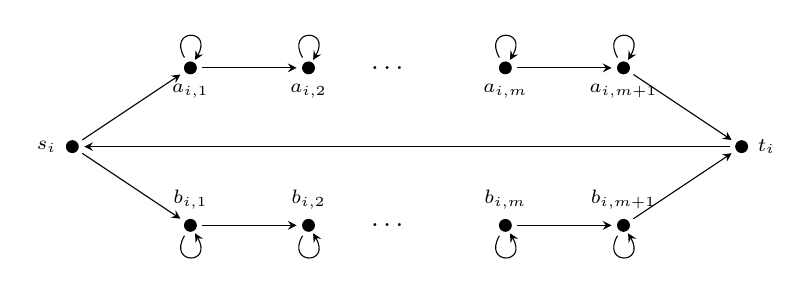
\begin{tikzpicture}[every edge/.style = {->, >=stealth,draw,auto,shorten <=2pt,shorten >= 2pt},
 vrtx/.style args = {#1/#2}{circle, draw, fill=black, inner sep=1.5pt,label=#1:{\scriptsize #2}}]

\node(u) [vrtx=left/$s_i$] at (-0.5,0) {};

\node(x1) [vrtx=below/$a_{i,1}$] at (1,1) {};
\node(y1) [vrtx=above/$b_{i,1}$] at (1,-1) {};

\node(x2) [vrtx=below/$a_{i,2}$] at (2.5,1) {};
\node(y2) [vrtx=above/$b_{i,2}$] at (2.5,-1) {};

\node at (3.5,1) {$\dots$};
\node at (3.5,-1) {$\dots$};

\node(xm-1) [vrtx=below/$a_{i,m}$] at (5,1) {};
\node(ym-1) [vrtx=above/$b_{i,m}$] at (5,-1) {};

\node(xm) [vrtx=below/$a_{i,m+1}$] at (6.5,1) {};
\node(ym) [vrtx=above/$b_{i,m+1}$] at (6.5,-1) {};

\node(v) [vrtx=right/$t_i$] at (8,0) {};
%
\path   (u) edge (x1)
        (u) edge (y1)
		(x1) edge [in=60,out=120,loop] (x1)
		(x2) edge [in=60,out=120,loop] (x2)
		(xm-1) edge [in=60,out=120,loop] (xm-1)
		(xm) edge [in=60,out=120,loop] (xm)
		(y1) edge [in=300,out=240,loop] (y1)
		(y2) edge [in=300,out=240,loop] (y2)
		(ym-1) edge [in=300,out=240,loop] (ym-1)
		(ym) edge [in=300,out=240,loop] (ym)
		(x1) edge (x2)
		(y1) edge (y2)
		(xm-1) edge (xm)
		(ym-1) edge (ym)
		(xm) edge (v)
		(ym) edge (v)
		(v) edge (u);

\end{tikzpicture}
\end{center}
The upper edges, i.e., $(a_{i,1},a_{i,2}),\ldots,(a_{i,m},a_{i,m+1})$, 
are called the {\em external ``true'' edges} of $x_i$,
and the lower edges, i.e., $(b_{i,1},b_{i,2}),\ldots,(b_{i,m},b_{i,m+1})$, the {\em external ``false'' edges} of $x_i$.

\paragraph*{Clause gadget.}
For each clause $C_j$, we have the following ``clause gadget'':
\begin{center}
\begin{tikzpicture}[every edge/.style = {->,> = stealth',draw,auto,shorten <=2pt,shorten >= 3pt},
 vrtx/.style args = {#1/#2}{circle, draw, fill=black, inner sep=1.5pt,label=#1:{\scriptsize #2}}]


\node(z) [vrtx=below/$z_{j}$] at (0,0) {};
\node(d) [vrtx=above/$d_{j}$] at (0,2) {};
\node(e) [vrtx=left/$e_{j}$] at (-2.5,-1.5) {};
\node(f) [vrtx=right/$f_{j}$] at (2.5,-1.5) {};
%

\path	(z) edge[<->] (d)
(z) edge[<->] (e)
(z) edge[<->] (f)
(e) edge[<->] (f)
(d) edge[bend right=45] (e)
(e) edge[bend right=45] (f)
(f) edge[bend right=45] (d);

\end{tikzpicture}
\end{center}
The ``outer'' edges $(d_{j},e_{j}),(e_{j},f_{j}),(f_{j},d_{j})$ are intended to represent the literals in $C_j$.
If $\ell_1,\ell_2,\ell_3$ are the literals in $C_j$,
then their associated edges are $(d_{j},e_{j}),(e_{j},f_{j}),(f_{j},d_{j})$, respectively.
To avoid clutter, we will call those edges $\ell_1$-edge, $\ell_2$-edge and $\ell_3$-edge, respectively.


\paragraph*{The XOR operator.}
We also have the ``XOR operator'' between two edges $(u_1,u_2)$ and $(v_1,v_2)$:

\begin{center}
\begin{tikzpicture}[every edge/.style = {->,> = stealth',draw,auto,shorten <=2pt,shorten >= 3pt},
 vrtx/.style args = {#1/#2}{circle, draw, fill=black, inner sep=1.5pt,label=#1:{\scriptsize #2}}]

\node(u1) [vrtx=left/$u_1$] at (-2,1) {};
\node(u2) [vrtx=right/$u_2$] at (6,1) {};

\node(z1) [vrtx=below/$\alpha_1$] at (0,0) {};
\node(z2) [vrtx=right/$\alpha_2$] at (2,2) {};
\node(z3) [vrtx=right/$\alpha_3$] at (2,-2) {};
\node(z4) [vrtx=below/$\alpha_4$] at (4,0) {};

\node(v2) [vrtx=left/$v_2$] at (-2,-1) {};
\node(v1) [vrtx=right/$v_1$] at (6,-1) {};

%

\path	(u1) edge (z1)
(z1) edge (v2)
(z1) edge[bend left=10] (z2)
(z2) edge[bend left=10] (z1)
(z1) edge node[below] {\tiny$-1$} (z3) 
(z2) edge[in=60,out=120,loop, min distance=1cm] node[above] {\tiny -1} (z2)
(z3) edge[in=300,out=240,loop, min distance=1cm] (z3)
(z2) edge[bend right=10] (z3)
(z3) edge[bend right=10] (z2)
(z3) edge[bend left=10] node[above] {\tiny 2} (z4)
(z4) edge[bend left=10] node[below] {\tiny 3} (z3)
(z1) edge node[above, at start,xshift=1cm,yshift=-0.1cm] {\tiny $-1$} (z4)
(z4) edge[bend right=10] (z2)
(z2) edge[bend right=10] (z4)
(z4) edge (u2)
(v1) edge (z4);

\end{tikzpicture}
\end{center}


\begin{definition}
\label{def:xor-graph}
Let $H$ be a graph, and let $(u_1,u_2)$ and $(v_1,v_2)$ are two non-adjacent edges in $H$.
\begin{itemize}
\item
For a cycle cover $R$ of $H$, we say that
{\em $R$ respects the property $(u_1,u_2)\oplus(v_1,v_2)$},
if $R$ contains exactly one of $(u_1,u_2)$ or $(v_1,v_2)$.
\item
Let $H'$ denotes the graph obtained from $H$ by replacing the edges $(u_1,u_2),(v_1,v_2)$
with the edges in the XOR operator above.

A cycle cover $R'$ of $H'$ is {\em an associated cycle cover} of $R$, if it satisfies the following condiiton.
\begin{itemize}
\item
If $R$ contains $(u_1,u_2)$,
then $R'$ contains a path from $u_1$ to $u_2$.
\item
If $R$ contains $(v_1,v_2)$,
then $R'$ contains a path from $v_1$ to $v_2$.
\item
$R\setminus \{(u_1,u_2),(v_1,v_2)\} \subseteq R'$.
\end{itemize}
\end{itemize}
\end{definition}


\begin{lemma}
\label{lem:xor-graph}
Let $H,H',R$ and $(u_1,u_2),(v_1,v_2)$ be as in Definition~\ref{def:xor-graph}.
Then, the following holds.
\begin{eqnarray*}
\sum_{R'\ \textup{is associated with}\ R} w(R') & = & 
\left\{
\begin{array}{ll}
4w(R), & \text{if}\ R \ \text{respects}\ (u_1,u_2)\oplus(v_1,v_2)
\\
0, & \text{otherwise}
\end{array}
\right.
\end{eqnarray*}
\end{lemma}



\paragraph*{Constructing the graph $G$.}
The graph $G$ is defined as the disjoint union of all the variable and clause gadgets
and the following additional edges to connect them:
For every clause $C_j$, for every literal $\ell$ in $C_j$,
if $\ell= x_i$, we ``connect'' the $\ell$-edge in the clause gadget of $C_j$
with the edge $(a_{i,j},a_{i,j+1})$ via the XOR operator;
and if $\ell= \neg x_i$, we ``connect'' it
with the edge $(b_{i,j},b_{i,j+1})$.

For an assignment $\phi:\{x_1,\ldots,x_n\}\to \{0,1\}$,
we say that {\em a cycle cover $R$ is associated with $\phi$}, if the following holds for every variable $x_i$.
\begin{itemize}
\item 
If $\phi(x_i)=1$, 
the cycle $(s_i,a_{i,1},\ldots,a_{i,m+1},t_i)$ is in $R$.
\item
If $\phi(x_i)=0$, 
the cycle $(s_i,b_{i,1},\ldots,b_{i,m+1},t_i)$ is in $R$.
\end{itemize}

\begin{lemma}
\label{lem:cycle-cover-assignment}
For every assignment $\phi:\{x_1,\ldots,x_n\}\to\{0,1\}$, the following holds.
\begin{eqnarray*}
\sum_{R \ \textup{is associated with}\ \phi} w(R) & = &
\left\{
\begin{array}{ll}
4^{3m}, & \text{if}\ \phi\ \text{is satisfying assignment for}\ \Psi
\\
0, & \text{if}\ \phi \ \text{is not}

\end{array}
\right.
\end{eqnarray*}
\end{lemma}


Combining Lemmas~\ref{lem:xor-graph} and~\ref{lem:cycle-cover-assignment},
it is immediate that the following holds.
\begin{eqnarray*}
\per(A) & = & 4^{3m}\times(\text{the number of satisfying assignments for}\ \Psi)
\end{eqnarray*}
Here $A$ is the adjacency matrix of $G$.



\section{Reduction from matrices over $\bbZ$ to matrices over $\{0,1\}$}
\label{sec:red-Z-to-01}

\paragraph*{Reduction to matrices over integers of the form $-2^k$, $0$ or $2^k$.}
For each edge $(u,v)$ with weight $2^{k}+ 2^{l}$,
we can replace it with $2$ ``parallel'' edges with weights $2^k$ and $2^l$, respectively.
\begin{center}
\begin{tikzpicture}[every edge/.style = {->,> = stealth',draw,auto,shorten <=2pt,shorten >= 3pt},
 vrtx/.style args = {#1/#2}{circle, draw, fill=black, inner sep=1.5pt,label=#1:{\scriptsize #2}}]


\node(u) [vrtx=left/$u$] at (0,0) {};
\node(v) [vrtx=right/$v$] at (4,0) {};

\node(z1) [vrtx=below/$z_1$] at (2,1) {};
\node(z2) [vrtx=above/$z_2$] at (2,-1) {};

\path	
(u) edge node[above] {\tiny $2^{k}$} (z1)
(u) edge node[below] {\tiny $2^{l}$} (z2)
(z1) edge (v)
(z2) edge (v)
(z1) edge[in=60,out=120,loop] (z1)
(z2) edge[in=300,out=240,loop] (z2);
%

\end{tikzpicture}
\end{center}

\paragraph*{Reduction to matrices over integers of the form $-1$, $0$ or $1$.}
For each edge $(u,v)$ with weight $2^{k}$,
we can replace it with $k$ ``series'' edges, each with weights $2$.
\begin{center}
\begin{tikzpicture}[every edge/.style = {->,> = stealth',draw,auto,shorten <=2pt,shorten >= 3pt},
 vrtx/.style args = {#1/#2}{circle, draw, fill=black, inner sep=1.5pt,label=#1:{\scriptsize #2}}]


\node(u) [vrtx=left/$u$] at (0,0) {};
\node(v) [vrtx=right/$v$] at (4,0) {};

\node(z1) [vrtx=below/$z_1$] at (1,0) {};
\node(z2) [vrtx=below/$z_2$] at (2,0) {};
\node(zk) [vrtx=below/$z_{k-1}$] at (3,0) {};

\node at (2.5,0) {$\dots$};

\path	
(u) edge node[above] {\tiny $2$} (z1)
(z1) edge node[above] {\tiny $2$} (z2)
(zk) edge node[above] {\tiny $2$} (v);
%

\end{tikzpicture}
\end{center}
Each weight $2$ edge can be further reduced to weight $1$ edge as above.


\paragraph*{Reduction to matrices over $\{0,1\}$ (but on modular arithmetic).}
The permanent of an $n\times n$ matrix $A$ over $\{-1,0,1\}$
can only in between $-n!$ and $n!$.
Let $m=n^2$.
Since $2^{m}+1 > 2n!$,
it is sufficient to compute $\per(A)$ in $\bbZ_{2^m+1}$.
Since $-1\equiv 2^m \pmod {2^m+1}$,
we can replace each~$-1$ with $2^m$, which can then be reduced to $1$ as above.

\section{$\sharpp$-hardness of $\perm$ -- Putting all the pieces together}

Putting together all the pieces from Sections~\ref{sec:red-sat-to-perm} and~\ref{sec:red-Z-to-01},
we design a polynomial time algorithm to compute $\sharp\threesat$
(with oracle access to language $O_{\per}$, i.e., the language associated with permanent).
On input 3-CNF formula $\Psi$, do the following.
\begin{itemize}
\item
Let $n$ and $m$ be the number of variables and clauses in $\Psi$.
\item
Construct a matrix $A$ over $\{-1,0,1\}$ such that $\per(A)$ is $4^{3m}$ times the number of satisfying assignments for $\Psi$.
\item
Let $m$ be an integer for which we can compute $\per(A)$ modulo $2^m+1$.
\item
Let $A'$ be the matrix obtained by replacing every $-1$ in $A$ with $2^m$. 
\item
Compute $\per(A')$ by querying the oracle on each bit.
\item
Let $Z$ be the remainder of $\per(A')$ divided by $2^m+1$.
\item
Divide $Z$ by $4^{3m}$ and output it.
\end{itemize}

\end{document}

%%%%%%%%%%%%%%%%%%%%%%%%%%%%%%%%%%%%%%%%%%%%%%%%%%%%%%%%%%%%%%%%%%%%%%%%%%%%%%%%%%%%%%
%%%%%%% END OF DOCUMENT %%%%%%%%%%%%%%%%%%%%%%%%%%%%%%%%%%%%%%%%%%%%%%%%%%%%%%%%%%%%%%
%%%%%%%%%%%%%%%%%%%%%%%%%%%%%%%%%%%%%%%%%%%%%%%%%%%%%%%%%%%%%%%%%%%%%%%%%%%%%%%%%%%%%%





